\documentclass[twocolumn,10pt]{article}

\usepackage[a4paper,hmargin=1.5cm,vmargin=2cm]{geometry}
\setlength{\columnsep}{0.7cm}
%\usepackage{microtype} % nice typesetting  % doesn't work for me :-( -S
\usepackage{amsmath}
\usepackage{graphicx}

\usepackage[utf8]{inputenc}
\usepackage{hyperref}
\urlstyle{same} % no tt font for URLs
\usepackage{natbib}
\bibliographystyle{genome_research}
\setlength{\bibsep}{0.3ex plus 0.2ex}
%\setcitestyle{aysep={}} 
\usepackage[dvipsnames]{xcolor}
\hypersetup{
    colorlinks,
    linkcolor={blue!50!black},
    citecolor={blue!50!black},
    urlcolor={blue!50!black}
}
\renewcommand{\topfraction}{0.9}
\renewcommand{\dbltopfraction}{0.9}
\renewcommand{\textfraction}{0.1}
\clubpenalty=1000
\widowpenalty=1000
\displaywidowpenalty=1000

\usepackage[compact]{titlesec}

\newcommand\blfootnote[1]{%
    \begingroup
    \renewcommand\thefootnote{}\footnote{#1}%
    \addtocounter{footnote}{-1}%
    \endgroup
}

\newcommand{\todo}[1]{[\textcolor{orange}{#1}]}

\begin{document}

\setcounter{secnumdepth}{0}

\twocolumn[{%
\centering
\textbf{\Large Analysing single-cell bisulfite sequencing data with \texttt{scbs}}\\[1.5ex]

Lukas P.~M. Kremer\textsuperscript{1,2,*}, Leonie Küchenhoff\textsuperscript{1,2}, Santiago Cerrizuela\textsuperscript{2}, Ana Martin-Villalba\textsuperscript{2}, Simon Anders\textsuperscript{1,*}\\[1ex]
{\footnotesize \textsuperscript{1} BioQuant Centre, University of Heidelberg, Heidelberg, Germany\\[-.5ex]
\textsuperscript{2} Molecular Neurobiology Dept., German Cancer Research Center (DKFZ), Heidelberg, Germany}
\vspace{1.5ex}

June 2022
\vspace{5.5ex}

\begin{minipage}{0.7\textwidth}
\small
\textit{Abstract} -- Single-cell-bisulfite sequencing (scBS) allows for assessing DNA methylation with single-basepair and single-cell resolution. Analysing the big data sets thus obtained requires preprocessing to reduce data size, improve signal over noise, and provide interpretability. Typically, this is simply done by dividing the genome into large tiles and averaging in these. We show that this coarse-graining dilutes signal, and suggest improved approaches to determine more informative regions quantify methylation in, and a better quantitation method than simple averaging. We demonstrate how our approach enables better distinguishing of cell types and reduces demands on cell number. We also show that our method of finding variably-methylated regions finds biologically meaningful loci. Finally, we present a software tool, \texttt{scbs}, that implements this approach and offers further functionality required to work with scBS data.
\end{minipage}
\vspace{6.5ex}

}]

\section{Introduction}

Sequencing-based assays with single-cell resolution have offered new means to understand the differences between the cells making up a sample. Single-cell RNA sequencing (scRNA-seq) techniques have matured at great pace in recent years, with well developed analysis methodology, and methods to study epigenetics at single-cell resolution are rapidly catching up. 
\blfootnote{\hspace{-.5cm}\raggedright\textsuperscript{*} e-mail:  \texttt{l.kremer@dkfz-heidelberg.de} and\\ \hspace{1cm}\texttt{simon.anders@bioquant.uni-heidelberg.de}}

Here, we discuss bisulfite sequencing, a method to study DNA methylation. In brief, DNA is treated with bisulfite, which converts unmethylated cytosines to uracils which are read as thymine in subsequent PCR, while methylated cytosines are protected from conversion. After sequencing, these conversions allow to determine the methylation status of all cytosines covered by reads \citep{Frommer_1992}. Bisulfite sequencing can also be performed with single-cell resolution \citep{Smallwood_2014} and even in parallel with scRNA-seq \citep{Clark2018}.

In the present paper, we discuss strategies to analyze scBS data, suggest improvement to current approaches, show their value in a benchmark, and present software to perform the improved analysis methods.

\subsection{Standard approach}

\begin{figure*}[t]
    \hspace{2.5cm}A\\[-7ex]
    \begin{center}
        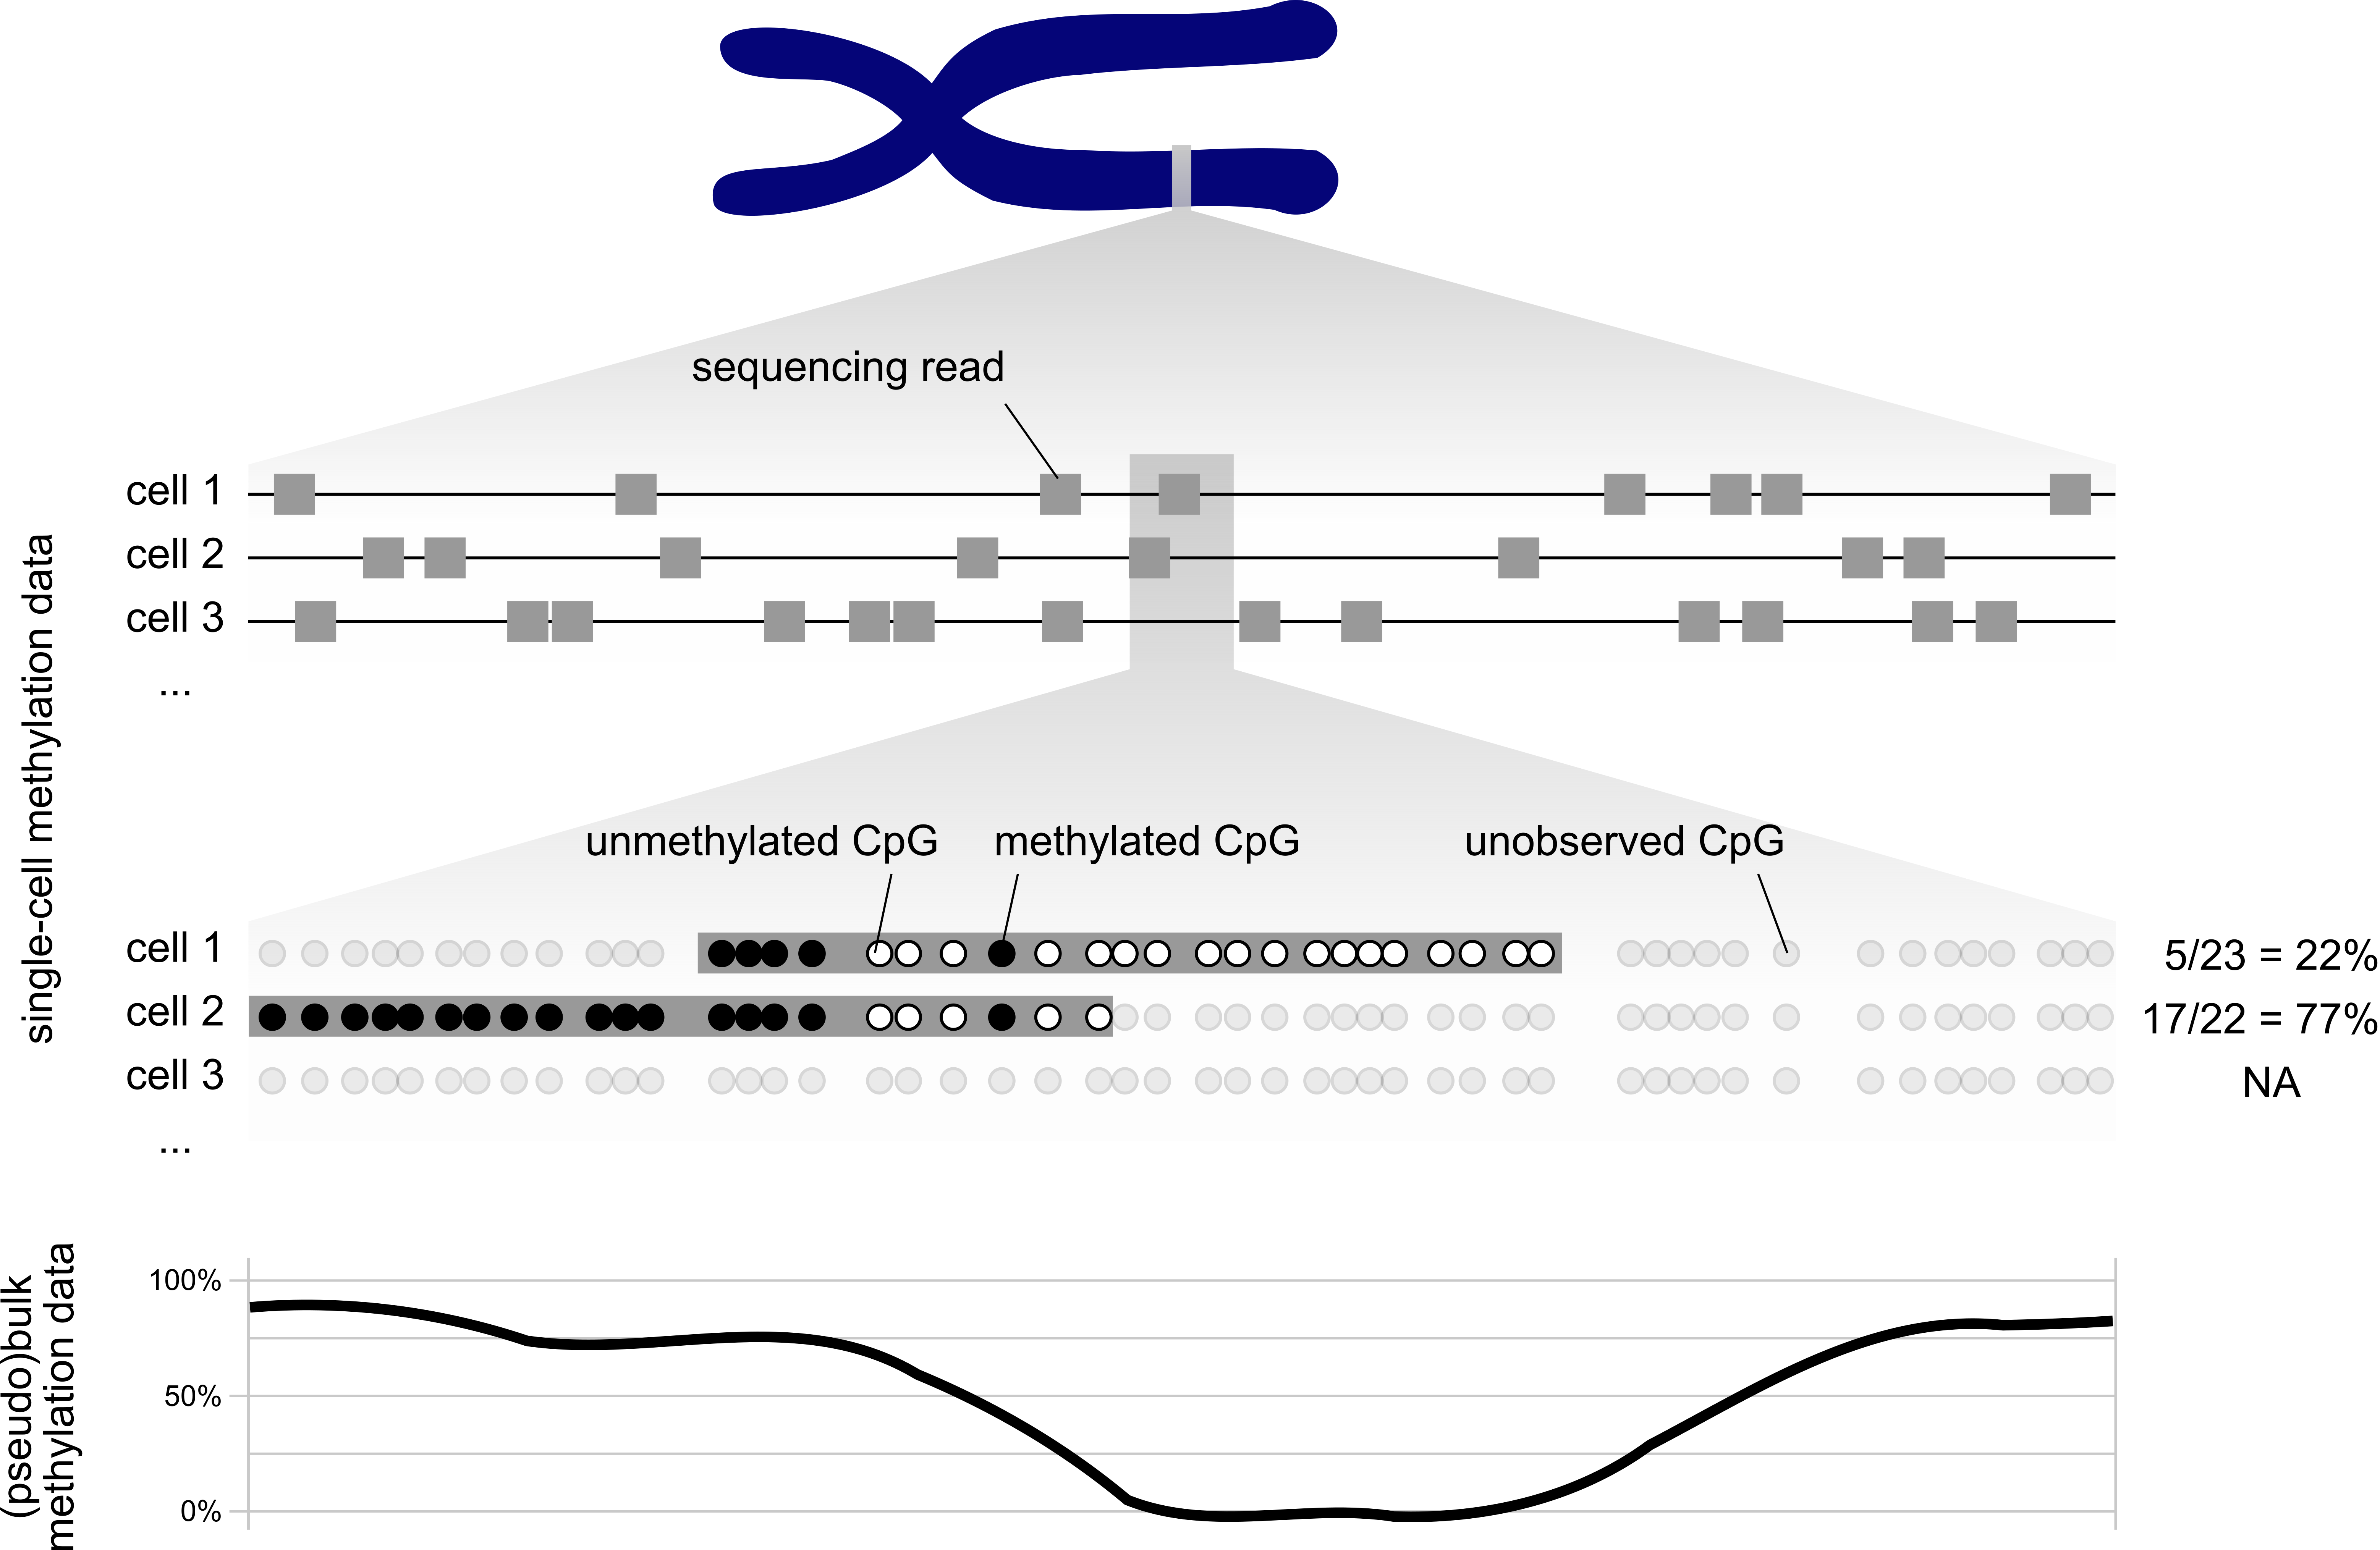
\includegraphics[width=0.7\textwidth]{figures/Fig_residuals_A.png}\\
    \end{center}
    \hspace{2.5cm}B\\[-3ex]
    \begin{center}
        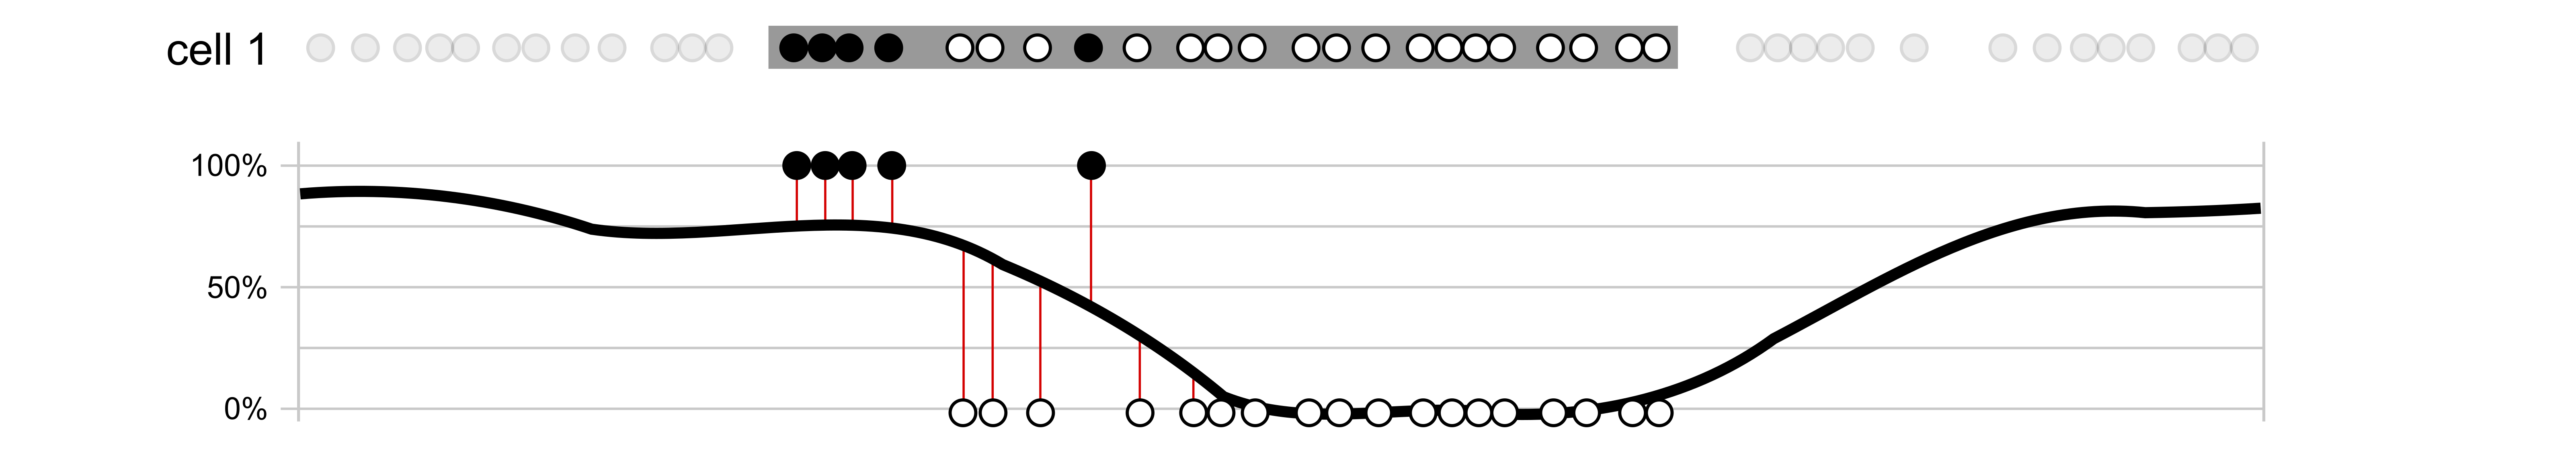
\includegraphics[width=0.7\textwidth]{figures/Fig_residuals_B.png}
    \end{center}
    \caption{\small \textbf{Effect of read position:} \textbf{(A)} Depicted is a genomic interval along a chromosome, for which DNA methylation is to be quantified. Two cells cover differing parts of the interval with one read each. If one simply counts for each cell which fraction of the covered CpG sites are methylated, one obtains very different values for the two cells. \textbf{(B)} By averaging each CpG site's methylation over all cells and subsequent smoothing, the thick black ``average methylation curve'' is obtained. To quantify the methylation of cell 1 from (A) relative to this average over all cells, we propose to use the cell's residuals to the smoothed curve (lengths of the vertical red lines) and take their average, counting residuals of methylated CpGs positive and residuals of unmethylated CpGs negative.}
    \label{fig:smoothres}
\end{figure*}


The standard approach to analyse scBS-Seq data is based on methodology developed for the analysis of single-cell RNA-Seq data. Therefore, we start by briefly reviewing how single-cell \emph{RNA}-Seq data is commonly analysed, before we discuss scBS data analysis.

The starting point in most scRNA-Seq analyses is a matrix of UMI counts (i.e. of counts of distinct RNA molecules), one row for each cell and one column for each gene. A first goal is usually to assigning cell types or states to cells. To this end, one needs to establish which cells are similar to each other, i.e., quantify the distance (i.e., dissimilarity) between any two given cells' transcriptional profile. A standard approach, used with minor variation in virtually all recent research and automated by popular software such as Seurat \citep{Hao_2021} or ScanPy \citep{Wolf_2018}, is as follows: One first accounts for cell-to-cell variation in sequencing depth by dividing each UMI count by the respective cell's total UMI count, then transforms to a homoskedastic scale by taking the logarithm. In order to avoid matrix elements with zero count to be transformed to minus infinity, one typically adds a very small ``pseudocount'' (often $10^{-4}$) to the normalized fractions before taking the logarithm. Now, one could use Euclidean distances of these vectors of logarithmized fractions as dissimilarity score. However, these scores would be exceedingly noisy due to the strong Poisson noise introduced by the many genes with very low counts. Therefore, one performs a principal component analysis (PCA), keeping only the top few (typically, 20 to 50) components. As Poisson noise is uncorrelated between genes, it will average out in the top principal components, as these are all linear combinations with weight on very many genes. Therefore, Euclidean distances between these ``PCA space'' vectors provide a robust dissimilarity score. Hence, the PCA space representation is suitable as input to methods like t-SNE and UMAP, which provide a two-dimensional representation of the data, or to methods for clustering (assigning cells to groups by similarity) and trajectory finding (identifying elongated manifolds in PCA space and assigning cells to quasi-1D positions along them).

This procedure is commonly adapted when working with single-cell DNA-methylation data, so that established methods used in scRNA-Seq can be used.
The task is therefore how to construct a suitable matrix as input for the PCA. A simple and common approach, used for instance by \citet{luo2017single}, is to divide the genome into tiles of, say, 100~kb size, and calculate for each cell the average methylation of the DNA within each tile. To this end, we identify all CpG sites in the tile for which we have coverage with at least one read and can hence call the CpG to be either unmethylated or methylated in the cell. Then we denote as average DNA methylation of this tile in a given cell the proportion of observed CpG sites in the tile that were found to be methylated (Figure \ref{fig:smoothres}A). This yields a matrix, with one row for each cell and one column for each genomic tile, comprising numbers (methylation fractions) between 0 and 1. This matrix is now subjected to PCA. After the PCA, one can proceed using approaches known from scRNA-seq.

While this simple procedure is straight-forward and produces satisfactory results, there is room for improvement. Here, we propose three improvements that, as we show afterwards, considerably increase the information content of the processed data. We will first explain the proposed improvement in a qualitative manner, while mathematical details are given later in the Methods section. Then, we will demonstrate the improvement using benchmarks.

\section{Improved processing of scBS data}

\subsection{Read-position aware quantitation} \label{residuals}

We first discuss the task of quantifying the level of methylation in a given, fixed, genomic interval. In Figure \ref{fig:smoothres}A, such an interval is covered by a single read for each of the two cells shown. The read from cell 2 shows much more methylation than the read from cell 1, and the standard analysis would therefore consider that cell as having stronger methylation in the interval. However, given that the two reads agree wherever they overlap, a more parsimonious interpretation would be that the cells do not show difference in methylation within the interval. Rather, both cells, and similarly maybe most other cells, might have stronger methylation in the left third of the interval than in the middle one.

Therefore, we propose to first obtain, for each CpG position, an average of the methylation across all cells and, then quantify for each individual cell its deviation from this average. In Figure \ref{fig:smoothres}B, the curved line depicts such an average over all cells, and the red vertical lines show an individual cell's deviation from the ensemble average. We take the lengths of the red lines as signed values (``residual''), positive for lines extending upwards from the curve (methylated CpG) and negative for lines extending downwards (unmethylated CpG), and take the average over the residual for all the CpGs in the interval that are covered by reads from this cell. In this average, we perform shrinkage towards zero via a pseudocount (to trade bias for variance, see Methods for detail) in order to dampen the signal in cells with low coverage of the interval.

The average thus obtained is what we use to quantify this cell's (relative) methylation in the interval. For a genome tiled into such intervals, we thus obtain a matrix, one row per cell, one column per interval, that can be used for downstream analysis, e.g., as input for a PCA. The signal to noise ratio in this matrix will be better than in a matrix obtained by simply averaging absolute methylation (0 or 1) over all the cells' covered CpG sites in a region. The reason for this is that we reduce the variation in situation as the one depicted in Figure \ref{fig:smoothres}A, where the methylation of the reads might differ strongly even though there is no actual evidence for a difference between the two cells.

How should one obtain the ensemble average (the curved line in Fig.\ \ref{fig:smoothres}B)? A simple approach to get a value for a specific CpG would be to take all cells with read coverage for the CpG and use the fraction of these that show the CpG as methylated. However, especially when only few cells offer coverage, these averages will be very noisy. Therefore, we propose to smoothen using a kernel smoother, i.e., by performing a kernel-weighted average over the CpG site's neighborhood. The kernel bandwidth (i.e., the size of the neighborhood to average over) is a tuning parameter; we got good results with 1000~bp and used this value for the examples presented here.

\subsection{PCA with imputation}

The standard PCA algorithm cannot deal with missing data. Therefore, one would need to make intervals wide enough to ensure that every interval is covered by at least one read for most tiles and discard any interval that is not covered by any single cell. Hence, a naive analysis has to resort to a coarse tiling of the genome. To counter this, we propose a simple and straightforward way to deal with missing data in the input matrix to a PCA: In a first iteration, we replace each missing value in the centered input matrix with zero, then run the PCA. Then, only these zeroes are replaced by the value predicted by the PCA and the PCA is rerun. Convergence is typically achieved after two to five iterations. For details, see Methods. 

The possibility to perform PCA with missing data allows us to use shorter, and thus more intervals and hence provide the PCA with richer input data.

\subsection{Finding variably methylated regions}

\begin{figure}
    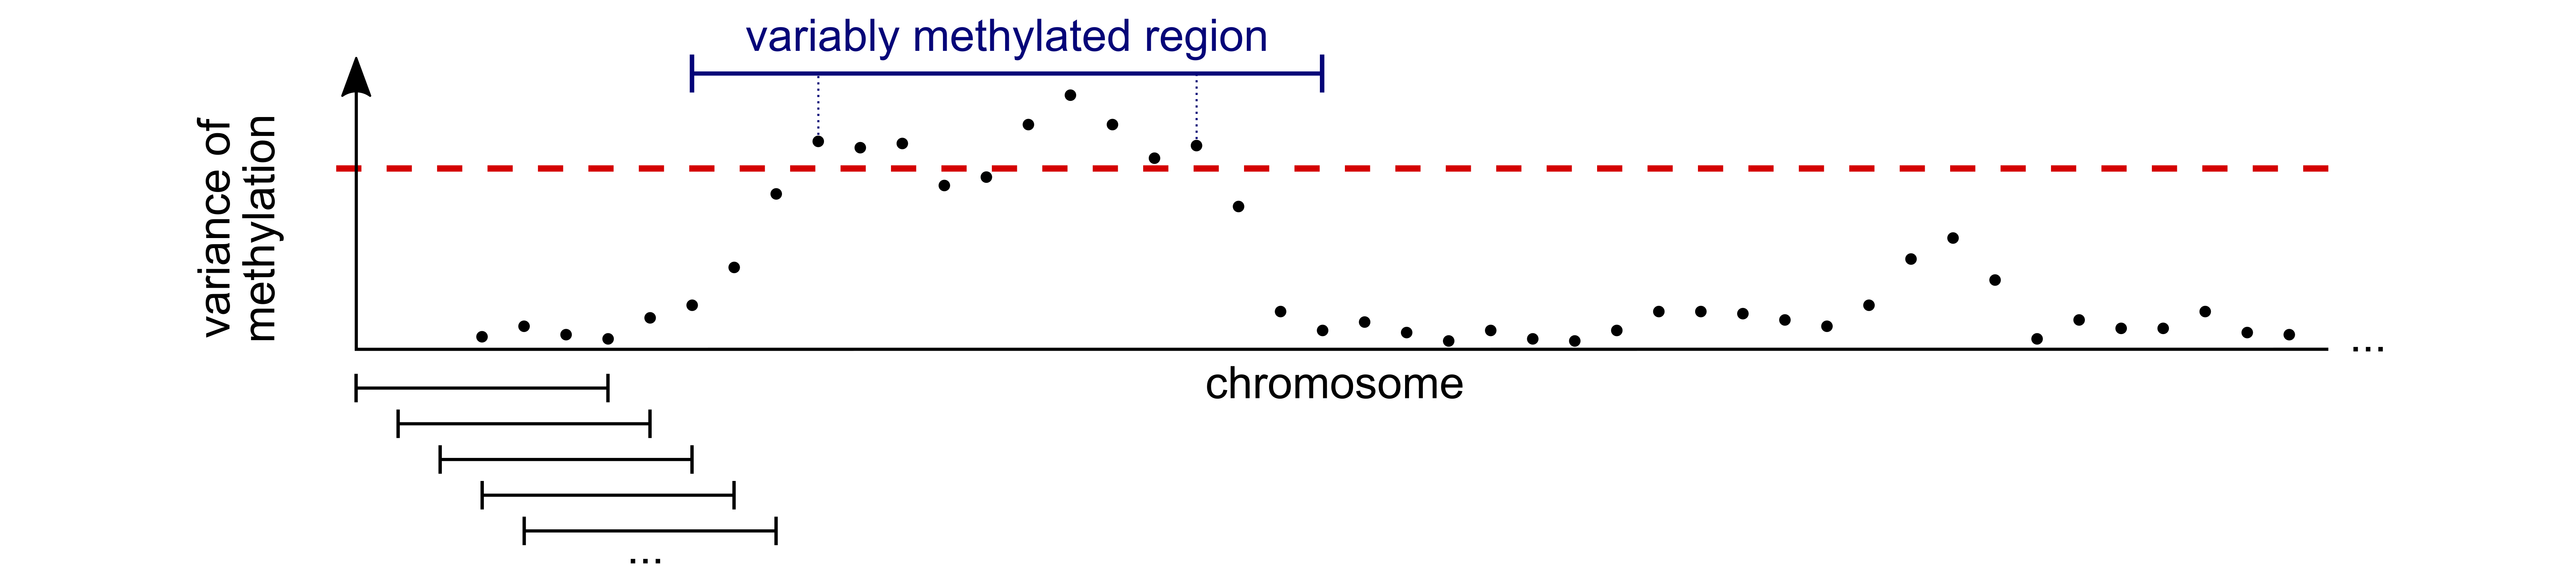
\includegraphics[width=\columnwidth]{figures/Fig_sliding.png}
    \caption{\small \textbf{Finding variably methylated regions (VMR):} The chromosomes are divided up into overlapping windows (first five shown at the bottom), and for each window, the cells' methylation values are calculated as described and as depicted in Fig.\ \ref{fig:smoothres}B. Then, the variance of these values is calculated (each point represents one of the overlapping windows), a threshold (dashed line) is chosen such that a chosen quantile of windows have a variance exceeding the threshold. Windows with above-threshold variance are merged if they overlap, yielding the ``variably methylated regions''.}
    \label{vmr}
\end{figure}


Typically, some regions in a chromosome will have very similar methylation status in all cells, while other regions show variability in methylation across cells. For instance, it is long known that CpG-rich promoters of housekeeping genes are unmethylated, and that a large proportion of the remaining genome is highly methylated regardless of cell type \citep{bird1986cpg}. In contrast, DNA methylation at certain genomic features such as enhancers is more dynamic \citep{argelaguet2019gastru}, and thus more variable across cells.
Only the latter regions are of value for our goal of quantitating dissimilarity between cells. We call these the variably methylated regions (VMRs).

In the standard approach, one divides up (tiles) each chromosome into non-overlapping, equal-sized intervals, and quantitates the methylation of each such tiles. Such rigid placing of interval boundaries is unlikely to be optimal: for example, a VMR might be much smaller than a tile and its signal will hence be drowned out by the larger part of uninformative CpGs that are equal in all cells, when averaging over all the CpG sites in the tile.

Therefore, we propose the following approach (Fig. \ref{vmr}): Divide up the chromosome into many \emph{overlapping} windows, that start at regular multiples of a fixed, small, step size. Quantify the methylation of each cell in each window by averaging the cell's methylation residuals over all CpGs in the window, as described above and depicted in Figure\ \ref{fig:smoothres}B. Then, calculate for each window the variance of these values over all cells. Select, say, the top 2\% windows with the highest variances and mark them as VMRs. Wherever thus marked windows overlap or are divided by only a small gap, merge them into one larger VMR. Then, calculate for each of these larger VMRs the methylation signal, as before, by averaging for each cell over the residuals of all contained CpG sites.

In this manner, we obtain a methylation matrix, with one row per cell and one column per VMR, that is, in a sense, richer in information and has better signal-to-noise ratio than the matrix obtained by the simple analysis sketched at the very beginning. As we demonstrate below, a PCA performed on such a matrix provided a distance metric for the cells that contains more information on biological detail than one from a simpler analysis. 

Besides providing better input for the distance calculations, the small size of identified VMRs also means that they can be readily compared with genomic annotation, which aids in their functional interpretation.
While a large 100~kb tile will often contain multiple genes with distinct expression patterns, small VMRs located in known regulatory elements or gene bodies are more easily associated with individual genes and their associated function.
Thus, VMRs provide a useful starting point for examining the data with methods from functional genomics.

\section{Benchmarks}

To demonstrate the value of our proposed improvements, we obtained two previously published scBS data sets and re-analysed them.

\subsection{Correlation with gene expression}

The first data set is a single-cell multi-omics data set generated by \citet{argelaguet2019gastru}. In their work, the authors obtained single-cell methylomes of mouse embryo cells across different stages of development (E4.5--E7.5) as well as single-cell transcriptomes from the same cells. In one of their analyses, the authors calculated the correlation between gene expression and promoter methylation to elucidate the implications of the epigenome on gene expression in development. The authors identified several genes where promoter methylation predicts gene expression, but obtained low correlations for the vast majority of genes. We reasoned that VMRs obtained with the previously described sliding window approach might be a better predictor of gene expression. 

In Figure \ref{figure:correlation}A, we compare correlations of gene expression and promoter methylation to correlations of gene expression and methylation of the closest VMR identified with \texttt{scbs scan}.
This analysis revealed a number of genes whose expression does not correlate with promoter methylation, but correlates with VMR methylation.
This effect is also observed when using our proposed measure of methylation, the shrunken mean of residuals (Figure \ref{figure:correlation}B).

\begin{figure}
    \begin{center}
    A\hspace{.9\columnwidth}~\\
    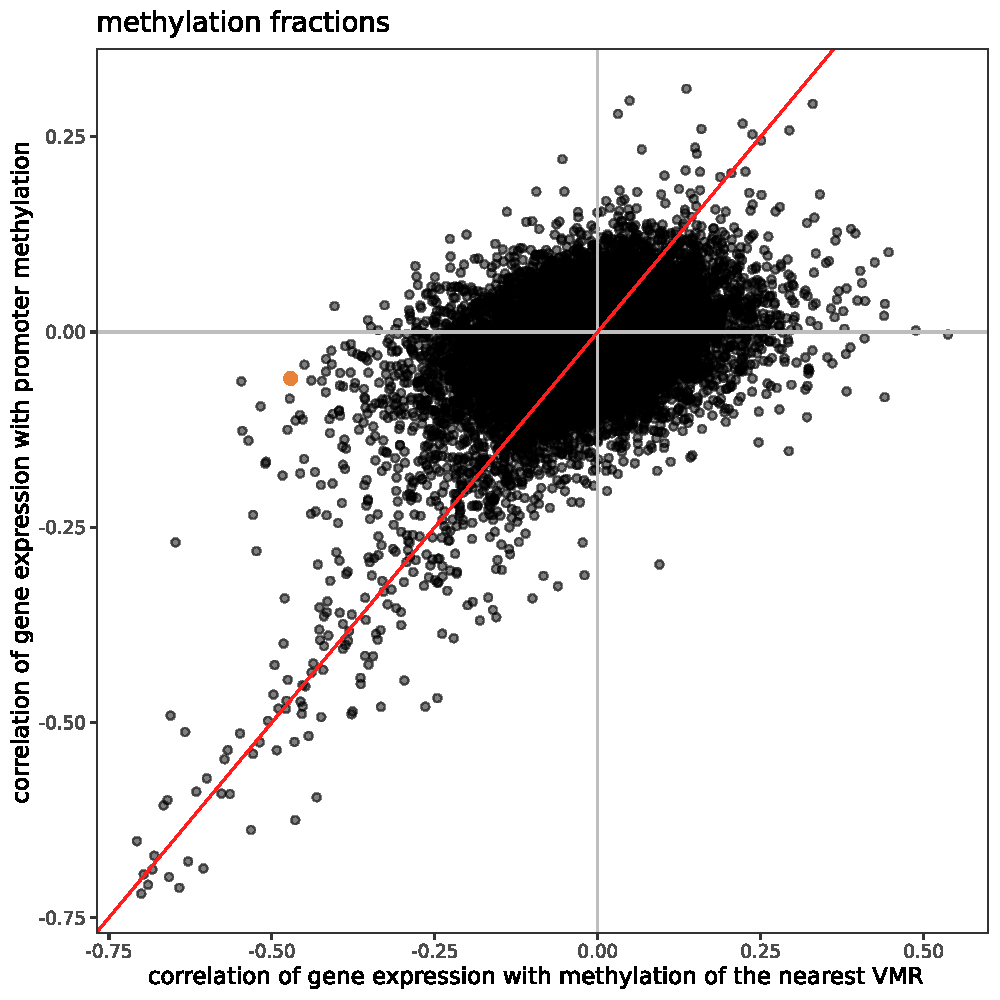
\includegraphics[width=.7\columnwidth]{part_leonie_git/leonie_plots/corr_methylation_fraction_4kbwindow.pdf} \\
    B\hspace{.9\columnwidth}~\\
    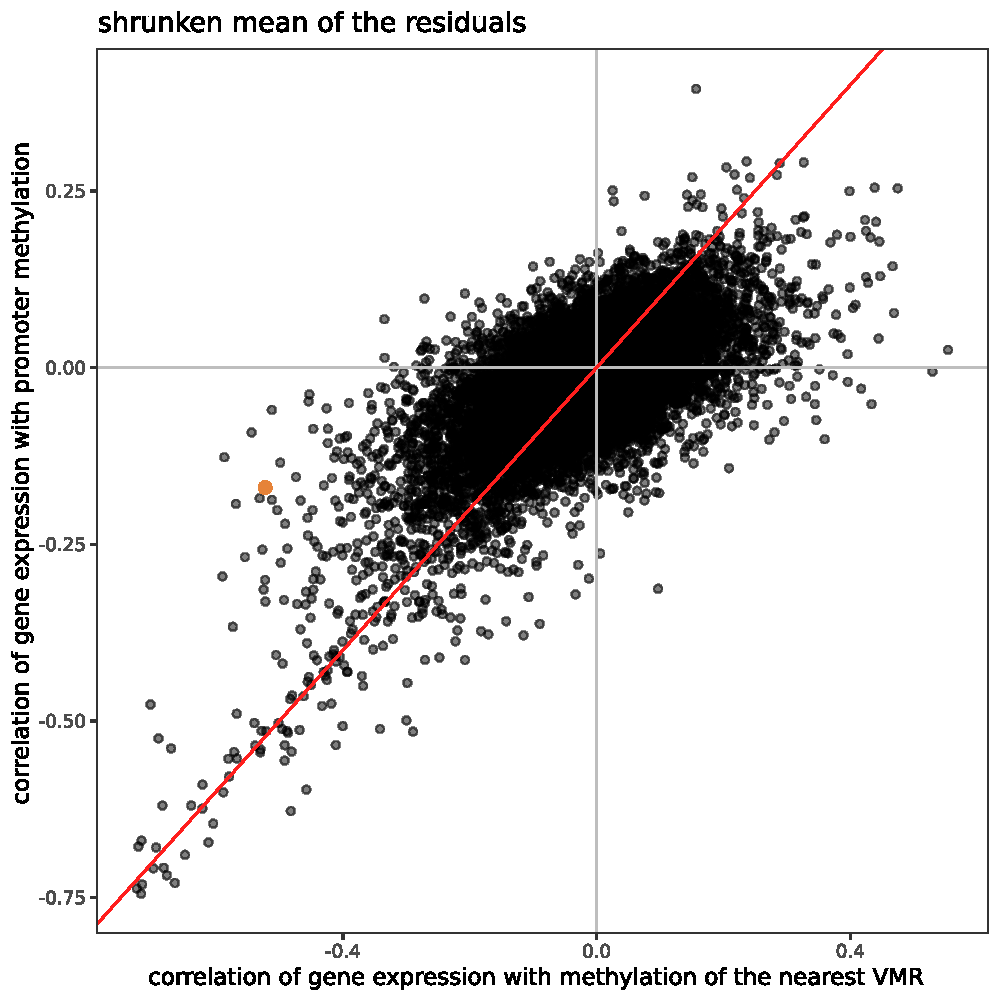
\includegraphics[width=.7\columnwidth]{part_leonie_git/leonie_plots/corr_shrunken_residual_4kbwindow.pdf} \\
    C\hspace{.9\columnwidth}~\\
    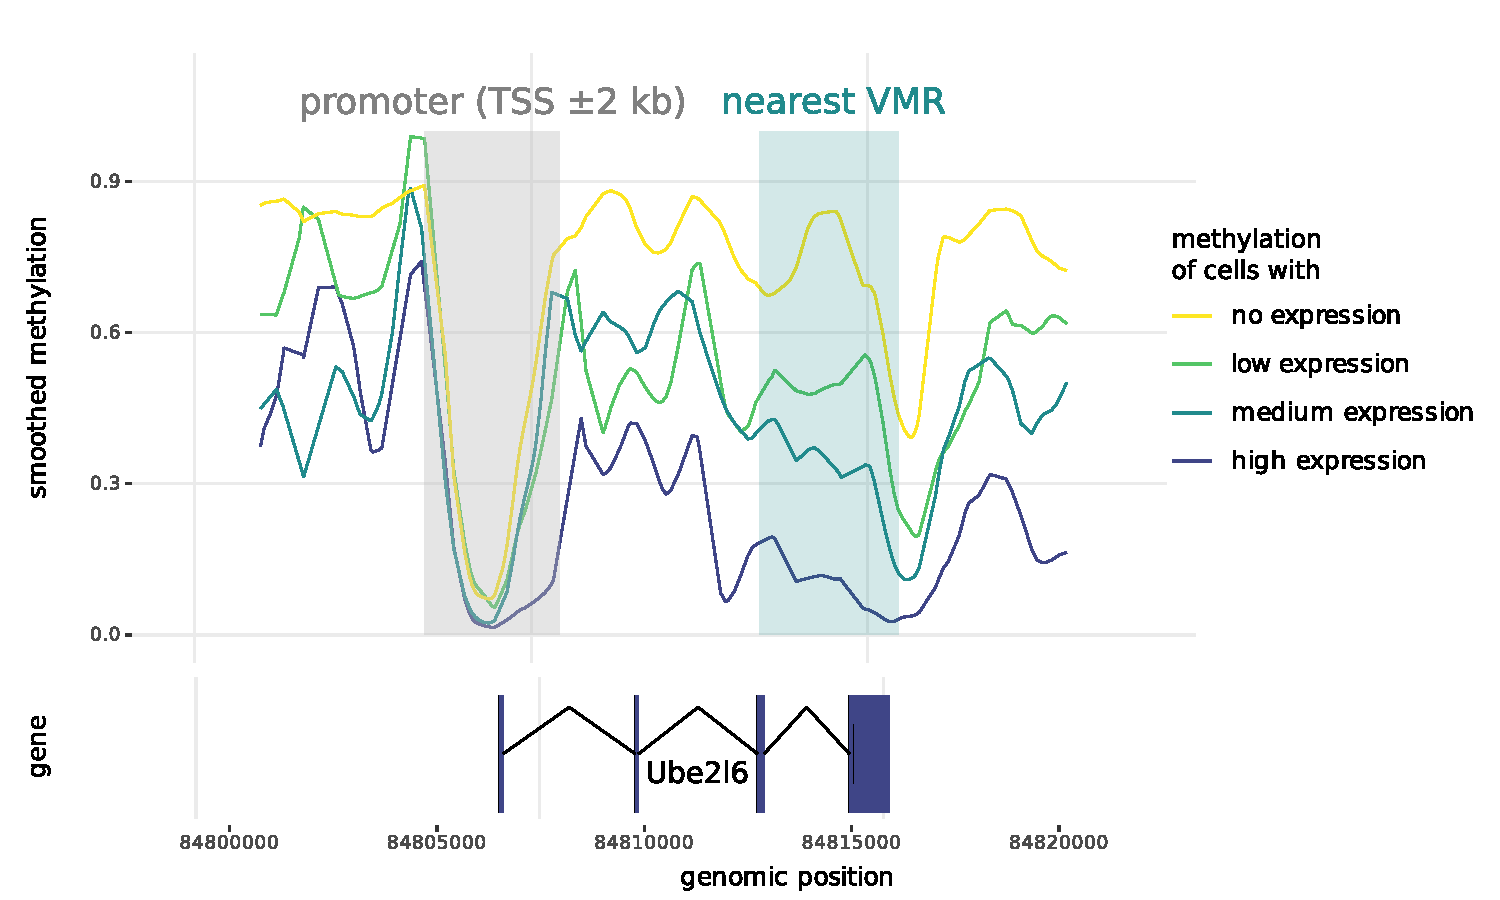
\includegraphics[width=.95\columnwidth]{part_leonie_git/leonie_plots/comparison_meth_RNA.pdf}
    \end{center}
    \caption{\small \textbf{Correlation of DNA methylation and gene expression}.
    \textbf{(A)} Correlation of each gene's RNA expression values to the the methylation fractions that were measured at promoters (y-axis), or to methylation fractions of the nearest VMR (x-axis). Promoters are defined as intervals \textpm2~kb around the TSS.
    \textbf{(B)} Same as in (A), but using mean shrunken residuals as a measure of methylation.
    \textbf{(C)} Mean smoothed methylation near the gene Ube2l6 (ENSMUSG00000027078, marked in yellow in A \& B). Cells are assigned to 4 groups based on Ube2l6 expression (group 0: cells with no Ube2l6 expression, groups 1-3: cells that express Ube2l6, divided into three equally large groups with group 3 having the highest expression). The mean methylation level of each group was smoothed with a tricube kernel of bandwidth 2000.
    Data from \citet{argelaguet2019gastru}.}
    \label{figure:correlation}
\end{figure}

To illustrate this effect with an example, we picked a gene where VMR methylation is a much better predictor of gene expression than promoter methylation (Ube2l6, highlighted in orange in Figure \ref{figure:correlation}A,B).
Grouping all cells into four groups according to their level of Ube2l6 expression, it is clearly visible that the promoter of this gene is lowly methylated regardless of gene expression, while methylation at the nearest VMR is greatly decreased in cells with high Ube2l6 expression.

\subsection{Identification of cellular sub-types}

\begin{figure*}
	\begin{center}
		A\hspace{.4\textwidth}B\hspace*{.3\textwidth}~\\
		\hspace{.3cm}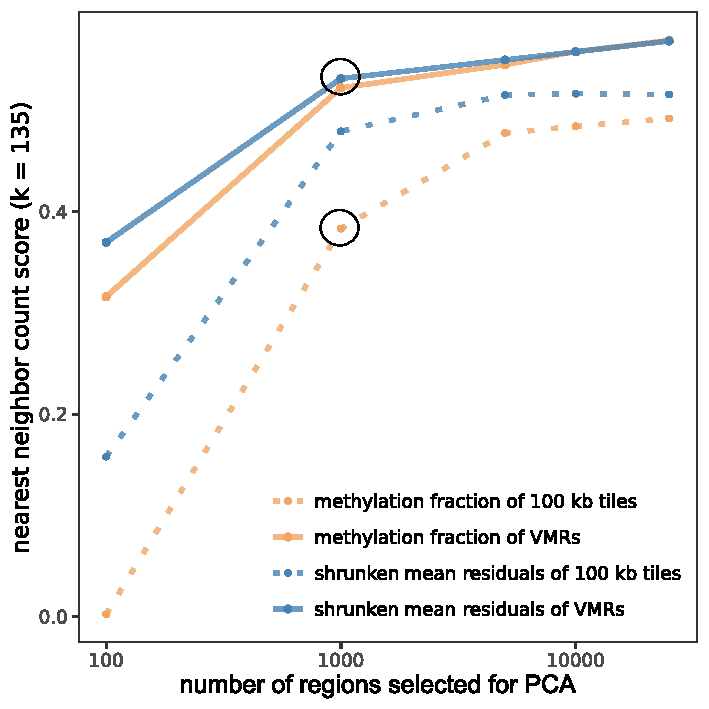
\includegraphics[width=.35\textwidth]{part_leonie_git/leonie_plots/complete_135k_12cm_log.pdf}
		\hspace{1cm}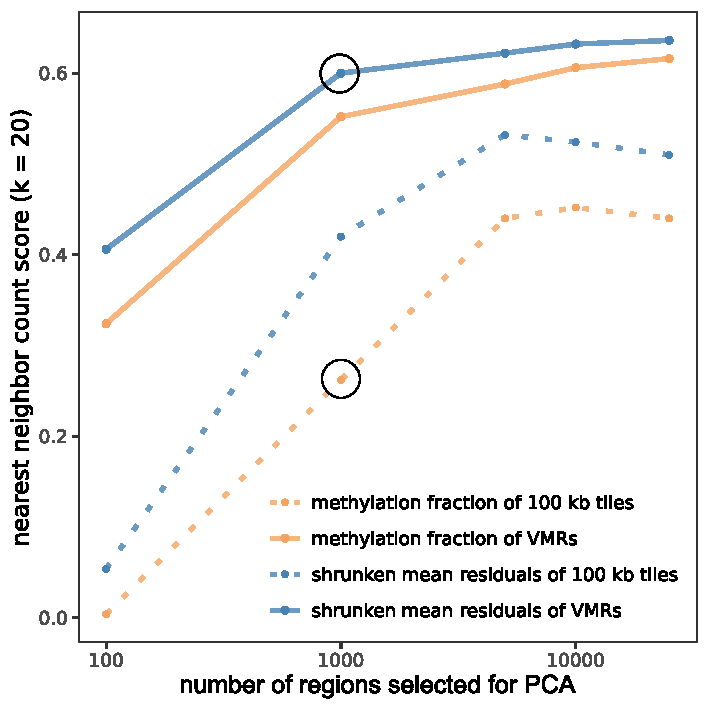
\includegraphics[width=.35\textwidth]{part_leonie_git/leonie_plots/cell500_20k_12cm_log.pdf}\\
		C\hspace*{.7\textwidth}~\\
		\hspace{.3cm}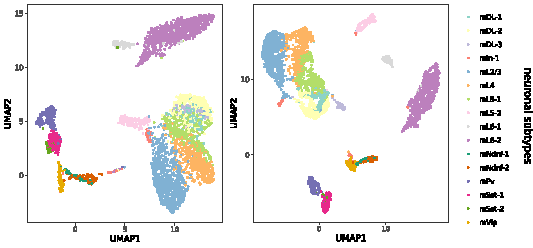
\includegraphics[width=.75\textwidth]{part_leonie_git/leonie_plots/UMAP_fulldataset.pdf}\\
		D\hspace*{.7\textwidth}~\\
		\hspace{.3cm}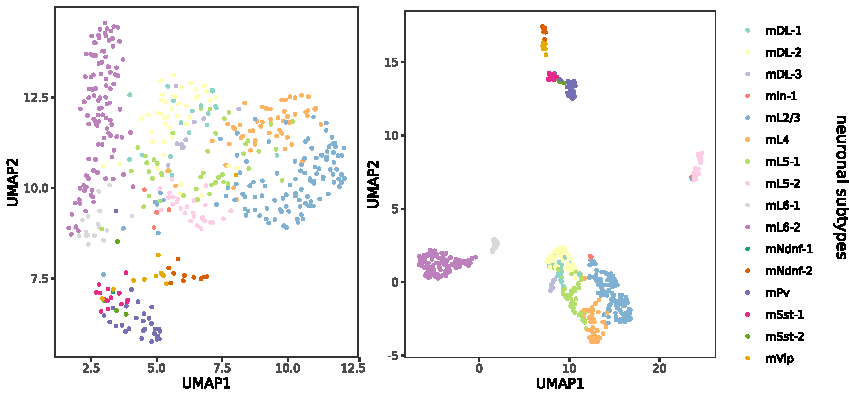
\includegraphics[width=.75\textwidth]{part_leonie_git/leonie_plots/UMAP_reduceddataset.pdf}
		\caption{\small \textbf{Benchmark of our methods on single-cell methylomes of 16 neuronal subtypes}. \textbf{(A)} Nearest neighbor count score using four different method combinations and a variable number of genomic regions (VMRs or 100~kb tiles) as input to PCA. Exemplary UMAPs for encircled analyses are shown in (C). \textbf{(B)} Same benchmark as in (A), but for a smaller data set consisting of 500 randomly subsampled cells. Exemplary UMAPs for analyses are shown in (D). \textbf{(C)} Two exemplary UMAPs of the full data set and methylation fractions of 100~kb tiles (left) or mean shrunken residuals of VMRs (right) \textbf{(D)} Two exemplary UMAPs of the smaller data set and methylation fraction of 100~kb tiles (left) or mean shrunken residuals of VMRs (right). Data from \citet{luo2017single}.}
		\label{figure:score}
	\end{center}
\end{figure*}

To assess the impact of our methods on dimensionality reduction and the ability to distinguish different (sub)types of cells, we used a data set from \citet{luo2017single}. This data set consists of 3377 single-cell CpG methylomes from the murine frontal cortex, comprising 16 neuronal subtypes.
We subjected this data set to the standard scBS workflow: defining a set of genomic intervals, quantifying methylation in these intervals, and subjecting the resulting matrix to PCA.
We repeated this analysis several times, either using 100~kb tiles or VMRs, and either using methylation fractions or mean shrunken residuals as a measure of methylation. 
For both types of regions, we varied the number of input regions, ranging from 100 to 50,000 high-coverage regions that were selected for PCA.
Specifically, we ranked regions by their number of coverging cells (i.e., cells with at least on read in the region) and selected those with the highest number.

To assess performance of each combination of methods, we used a nearest neighbor count score (see Methods) that quantifies how well the different neuronal subtypes are separated in 15 dimensional PC space. We used the original assignment of cells to cell types from \citet{luo2017single}.
The results demonstrate that the 16 neuronal subtypes are more cleanly separated when using our proposed methods (Figure \ref{figure:score}A).
Most of this gain in performance can be attributed to the use of VMRs over genomic tiles. The use of mean shrunken residuals over methylation fractions provides an additional small improvement.

Since scBS protocols is still rather costly and labor-intensive, only few laboratories are currently able to obtain thousands of single cell methylomes.
To simulate a smaller data set, we subsampled the frontal cortex data set to 500 cells and repeated our analysis.
Here, our approach keeps its good score, while the simple approach falls behind (Figure \ref{figure:score}B).

Of note, our results show that even few VMRs (here, the 1000 VMRs that have read coverage in the highest number of cells) already contain sufficient information to distinguish neuronal subtypes.
In contrast, the neighbor count score for the top 1000 genomic 100~kb tiles is much lower.
To visualize the different degrees of separation, we further reduced the PC space from both analyses with UMAP, showing that some neuronal subtypes such as mL5-1 and mDL-3 are separated from the other subtypes when using 1000 VMRs (Figure \ref{figure:score}C).
% why not just plot PC1 vs. PC2 here? % because people will want to see the UMAP. -S
Again, the difference is even more pronounced in the sub-sampled analysis with only 500 cells (Figure \ref{figure:score}D).

\section{The \texttt{scbs} Python package}

\begin{figure*}[t]
	\begin{center}
		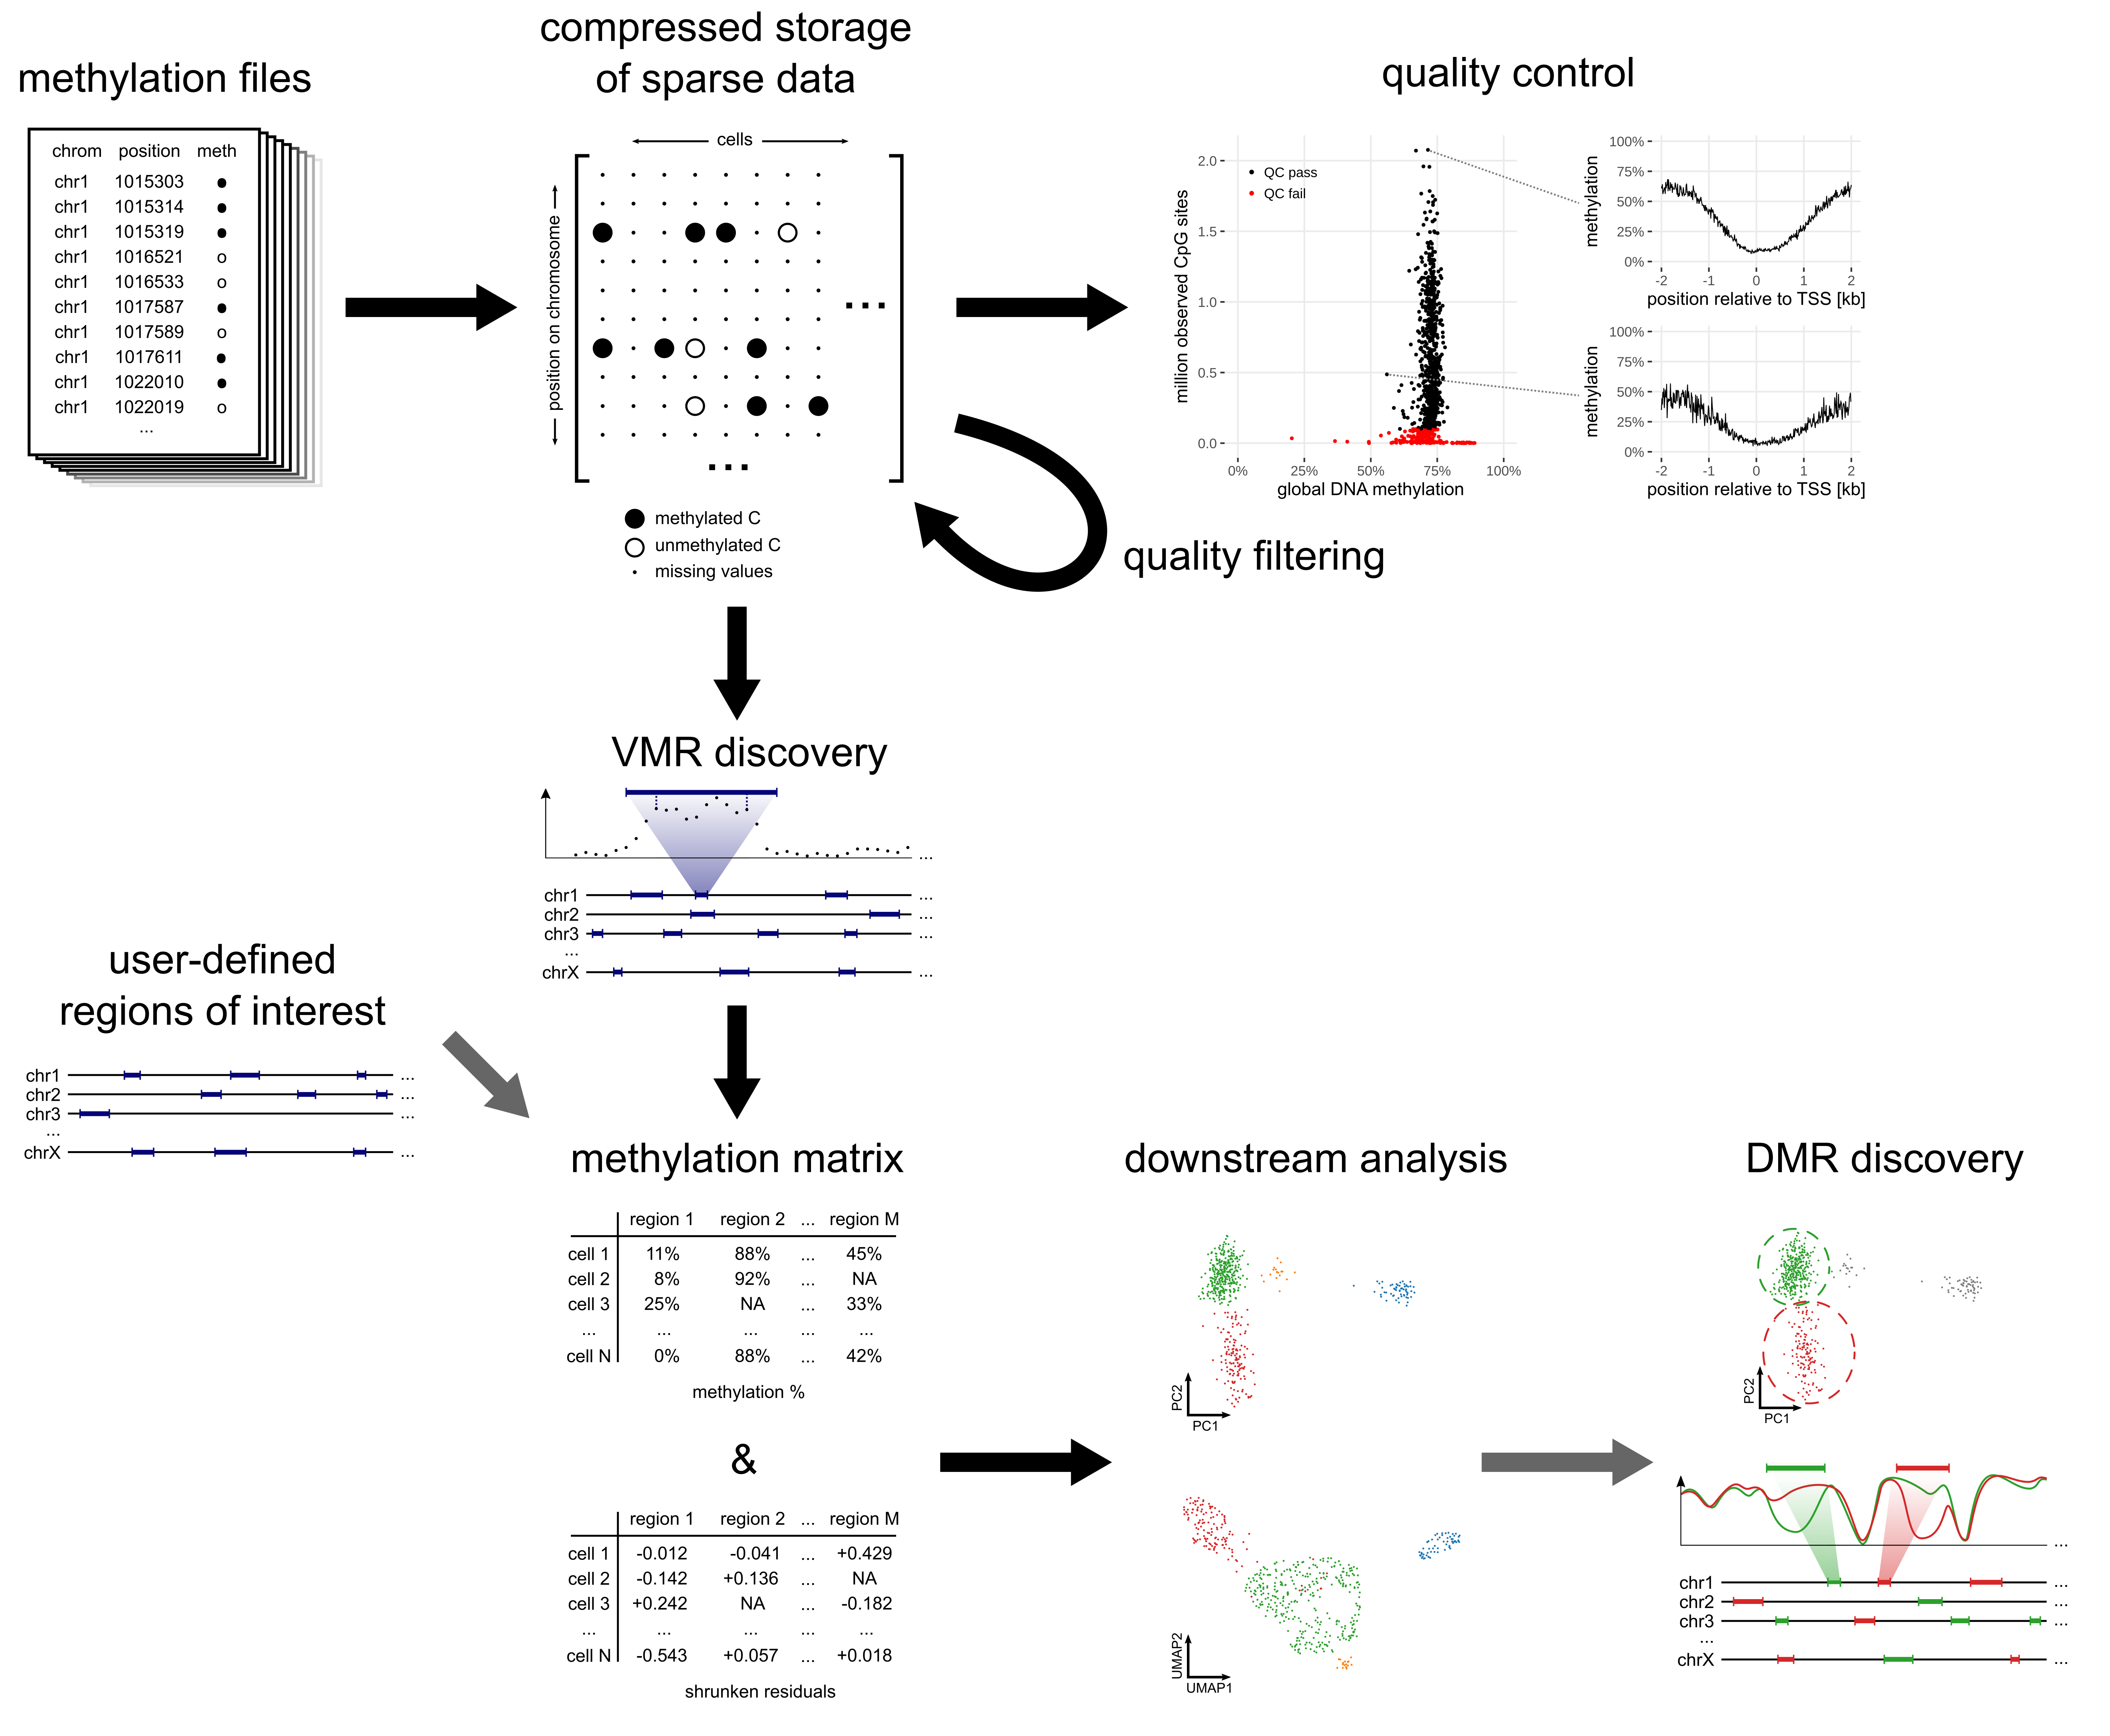
\includegraphics[width=.8\textwidth]{figures/Fig_workflow.png}
	\end{center}
	\caption{\small \textbf{Overview of the functionalities implemented in the \texttt{scbs} package.}
		\texttt{scbs prepare} parses methylation files produced by common bisulfite sequencing mappers and stores their contents in a compressed format optimised for efficient access to genomic intervals.
		\texttt{scbs} also produces cell-wise summary statistics and quality plots (here: average methylation around the transcription start site) that are used to detect low-quality cells.
		These cells can be discarded with \texttt{scbs filter}.
		To obtain a methylation matrix, similar to the count matrices used in scRNA-seq, the user must first decide in which genomic intervals methylation should be quantified.
		The user may either provide genomic regions of \emph{a priori} interest, or they may choose to discover VMRs (variably-methylated regions) in the data with \texttt{scbs scan}.
		The resulting methylation matrix can then be used for downstream analysis such as cell clustering and dimensionality reduction.
	}
	\label{workflow}
\end{figure*}

We have implemented the approach just described in a Python package with a command line interface, called \texttt{scbs}, which also offers a number of other functionalities for the analysis of scBS data (Figure \ref{workflow}). The starting point of such an analysis are methylation files generated by tools such as Bismark \citep{bismark} or methylpy \citep{methylpy}. For each cell, these tools produce a text file that lists the methylation status of all CpG sites. Since it is inconvenient to work with hundreds or thousands of text files, \texttt{scbs} provides the \texttt{prepare} command which parses these methylation files and stores their content in a compressed format that enables efficient access to all CpG sites of the genome. \texttt{scbs prepare} is flexible and accepts all tabular input formats including Bismark .cov-files, methylpy .allc-files, or custom user-defined formats.

In brief, we store methylation of each chromosome in a matrix where each column represents a cell and each row represents a base pair. Methylated and unmethylated sites are coded as $+1$ and $-1$, respectively. Since the vast majority of values in this matrix are missing due to the sparsity of scBS data (and because rows for base-pairs not corresponding to a CpG site contain no data), we encode missing values as zero and then store the data in Compressed Sparse Row (CSR) format. This format does not explicitly store zeroes (here: missing values) and is optimized for row-wise access, which results in significant compression and allows fast access to the methylation status of genomic intervals.

\texttt{scbs prepare} also computes a number of summary statistics for each cell, including the mean genome-wide methylation level and the number of observed CpG sites, i.~e. the number of CpG sites that have sequencing coverage. These summary statistics can be used to detect cells with poor quality. The quality of each single cell methylome can furthermore be inspected with \texttt{scbs profile}, which computes the average methylation profile of a set of user-defined genomic regions such as transcription start sites (TSS) at single-cell resolution. The TSS profile is a useful quality control plot since methylation shows a characteristic dip roughly \textpm1~kb around the transcription start site in mammalian genomes. Cells that do not show this pattern, or cells with few observed CpG sites, may then be discarded with \texttt{scbs filter}. 

After quality control, the user has access to the genome-wide VMR detection approach described above via \texttt{scbs scan}. This produces a BED file that lists the genome coordinates of VMRs. To finally obtain a methylation matrix analogous to a scRNA-seq count matrix, this BED file can be used as input for \texttt{scbs matrix}, which quantifies methylation at genomic intervals in all cells. The command produces both the percentage of methylated CpG sites, as well as our proposed methylation measure (shrunken mean of the residuals) that is more robust to variation in sequencing coverage or stochastic differences in read position between cells. We note that both \texttt{matrix} and \texttt{profile} accept any valid BED-file as input, which means that the user can quantify and visualize methylation at any genomic feature of interest, such as promoters, enhancers or transcription factor binding sites, in single cells. The obtained methylation matrix can then serve as input for common single-cell analysis methods such as dimensionality reduction and cell clustering.

\texttt{scbs} is free and open source, and the package can be installed via the Python package manager. The source code and the package are available at \href{https://github.com/LKremer/scbs}{https://github.com/LKremer/scbs}, where we also provide detailed documentation including a tutorial that demonstrates a complete \texttt{scbs} analysis on an example data set.




\section{Discussion and Conclusion}

Here, we have proposed an improved strategy to preprocess single-cell bisulfite-sequencing data.
Based on the observation that incomplete read coverage of a genomic interval can lead to inaccurate methylation estimates, we suggest a scoring scheme that is aware of a reads local context rather than just treating all reads in an interval alike
Furthermore, we show a way to pinpoint minimal regions of high variability across cells, which we call variably-methylated regions (VMRs).
By reanalyzing two published datasets we could show that these improvements to data preprocessing help to increase signal and decrease noise, resulting in a more informative intermediate-dimensional representation of the data. As examples of practical benefits, we demonstrate that our preprocessing allows for better distinction of cell sub-types, especially for smaller data sets with limited numbers of cells. In addition to this improvement of global signal-to-noise ratio (with regards to cell dissimilarity quantification), we also show that the determination of VMRs improve biological interpretability by pinpointing the regions that actually change and hence have a putative regulatory role.

Furthermore, we have presented and published an open source software tool, called \texttt{scbs}, that provides an easy-to-use implementation of the described algorithms. The package also offers functionality for all other steps of data preprocessing that are needed to get from the output of methylation callers such as Bismark and methylpy to a cell\texttimes region matrix that is suitable as input for standard analysis tools that work in a reduced-dimensionality setting, thus allowing the user to use, e.g., well established tools from scRNA-seq analysis, including visualization tools such as t-SNE and UMAP, Leiden/Louvain clustering, pseudotime trajectory analyses etc. By offering these functions, \texttt{scbs} bridges a gap in the chain of existing tools that so far hindered practitioners in their data analysis.

In addition, by pinpointing exact regions of interest, the VMR functionality provides useful input for genomics-style analyses.
Depending on the research question at hand, individual VMRs can be related to nearby genomic features such as gene bodies or known regulatory elements, tested for methylation differences between groups of cells, or subjected to gene ontology enrichment or motif enrichment.

In conclusion, we have presented powerful improvements to scBS data preprocessing and a software tool that implements these and also completes a gap in existing tool chains.

\vspace{1.4ex}
\noindent\hfil\rule{.6\columnwidth}{.2pt}\hfil

\section{Methods}

\subsection{Raw data}

We write $x_{ij}$ for the methylation status of CpG $i$ in cell $j$. The index $i$ runs over all CpG positions present in the genome, the index $j$ over all cells in the assay. We write $x_{ij}=0$ if position $i$ was found to be unmethylated in cell $j$ by bisulfite sequencing , $x_{ij}=1$ if it was methylated, and $x_{ij}=\text{NA}$ if position $i$ was not covered by reads from cell $j$ and the methylation status is therefore not available ("NA"),

These values can be readily obtained from single-cell bisulfite sequencing data using tools like Bismark.

If multiple reads with the same cell barcode cover the positions, these will typically be PCR duplicates of each other and hence agree. Of course, the two alleles of a CpG may differ in their methylation status and while it is in principle possible that one obtains reads stemming the same position on both the paternal and the maternal chromosomes of the same cell, but this is so unlikely that we can ignore the case. Hence, whenever Bismarck reports multiple reads covering the same position in the same cell, we set $x_{ij}$ to 0 or 1 following the majority of reads and put $x_{ij}=\text{NA}$ in case of a tie. 

For later use: We write $C$ for the set of all cells in the assay (i.e., $C$ is the index set for the cell indices $j$). Moreover,
we define $C_i\subset C$ as the set of all those cells $j$ that have reads covering position $i$,
$$ C_i=\{j\in C: x_{ij}\neq\text{NA}\}.$$
Conversely, we define $G_j$ as the set of all the CpG positions $i$ covered by reads from cell $j$ 
$$ G_j=\{i: x_{ij}\neq\text{NA}\}.$$

\subsection{Data storage}

The function \texttt{scbs prepare} reads a set of methylation files (e.g. produced by Bismark) and produces a file that stores the matrix $x$ in a space-efficient format, as follows: $x$ is represented as a SciPy sparse matrix \citep{SciPy}, encoding the actual values 0, 1, and NA as -1, 1, and 0, respectively. Coding NA (the most common value) as 0 leverages SciPy's sparse matrix storage. In all the follows here, any mention of $x$ will, however, always mean the encoding as $x_{ij}\in\{0,1,\text{NA}\}$.

\subsection{Smoothing}

For each CpG position $i$, we write 
$$\overline{x}_i=\langle x_{ij} \rangle_{j\in C_i} = \frac{1}{|C_i|}\sum_{j\in C_i} x_{ij}$$ 
for the average methylation at position $i$, where $\langle\cdot\rangle$ denotes averaging, and the average runs over all the cells $j\in C_i$, i.e. over those cells for which methylation data is available for position $i$.

%\todo{NOTE: Here, we could already do shrinkage and use $\frac{1}{|C_i|+1}\sum_i x_{ij}$ instead. But we don't do that, right?}

We then run a kernel smoother over these per-position averages to obtain the smoothed averages $\tilde x_i$. Specifically, we use
\[ \tilde x_i = \frac{\sum_{i'} \overline x_{i'}\, k_h(d_{ii'})}{\sum_{i'} k_h(d_{ii'})},\]
i.e., $\tilde x_i$ is the weighted average over the per-position averages $\overline{x}_{i'}$, taken over the CpG sites $i'$ in the neighborhood of $i$, and weighted using a smoothing kernel $k_h$ with bandwidth $h$. Here, $d_{ii'}$ is the distance between CpG positions $i$ and $i'$, measured in base pairs, $h$ is the smoothing bandwidth in base pairs (by default, $h=1000$), and $k_h$ is the tricube kernel,

\[ k_h(d) = \left\{
\begin{aligned}
    &\left(1-|d/h|^3\right)^3 &\text{for } |d|<h \\
    &\,0 &\text{otherwise}. 
\end{aligned}
\right.
\]

\subsection{Methylation for an interval}

Next, we discuss averaging methylation over a range of CpG sites.

Given an interval $I$ on the chromosome, we wish to quantify the average methylation $m_{Ij}$ of the CpG sites within the interval for cell $j$. If we interpret $I$ as the set of CpG positions $i$ in the interval, we may write

$$ m_{Ij} = \left< x_{ij} \right>_{i\in I\cap G_j}.$$

Here, the average runs over all those sites $i$ that lie within the interval $I$ and are covered by reads from cell $j$.

If we wish to compare cells, it can be helpful to center this quantity by subtracting its average:

$$ z_{Ij} = m_{Ij} - \langle m_{Ij'}\rangle_{j'\in C}.$$

As an alternative, we suggest to consider the residuals of the individual CpG methylation values $x_{ij}$ from the smoothed average $\tilde x_i$,
$$ r_{ij} = x_{ij} - \tilde x_i, $$
and averaging over these, obtaining
\begin{equation} 
r_{Ij} = \frac{\scriptsize{1}}{\scriptsize{|I\cap C_i|+1}}\sum_{i\in I\cap C_i}\left( x_{ij} - \tilde x_i \right). \label{avgres}
\end{equation}

This is a shrunken average, with denominator $n+1$. This extra pseudocount has the effect of shrinking the value towards the "neutral" value 0, with the shrinkage becoming stronger if the data is "weak" because the number $|I\cap C_i|$ of positions covered by reads from cell $j$  is low. In the extreme case of none of the reads from cell $j$ covering $I$, the sum becomes 0 and the denominator 1, i.e. $r_{Ij}=0$ in this case.

\subsection{Finding variably methylated regions (VMRs)}

For any interval $I$, we denote by $v_I$ the variance of its residual averages $r_{Ij}$:

$$ v_I = \frac{\scriptsize{1}}{\scriptsize{|C_I|}}\left( r_{Ij} - \langle r_{Ij'}\rangle_{j'\in C_I} \right)^2,$$

where the average runs only over the set $C_I=\bigcup_{i\in I}C_i$ of those cells $j$ which have reads covering interval I.

To find VMRs, we define intervals $I_1, I_2, ...$, all of the same width, and with step-wise increasing starts, then calculate $v_1, v_2, ...$ for these intervals. We then mark the intervals with the 2\% highest variances. We take the union of all these intervals, split the union into connected components, and call each component a VMR. Putting that last step in other words: We take all the intervals with variance in the top 2-percentile, fuse intervals that overlap and call the regions thus obtained the VMRs.

\subsection{Calculating cell to cell distances}

Given a set, $\mathcal{V}=\{I^\text{v}_1,I^\text{v}_2,\dots\}$, of intervals corresponding to VMRs, we get a relative methylation fraction $r_{ij}$ for each VMR $I^\text{v}_i$ and each cell $j$ from Eq.\ ()\ref{avgres}). The matrix thus obtained can then be centered and used as input for a PCA. If we calculate the top $R$ principal components, we thus obtain for each cell $j$ an $R$-dimensional principal component vector $\mathbf{x}^\text{P}_j$. For any two cells $j$, $j'$, we use the Euclidean distance $\|\mathbf{x}^\text{P}_j - \mathbf{x}^\text{P}_{j'}\|$ as the measure of dissimilarity of the two cells.
Thus, the matrix of PC scores can be used as input to dimension reduction methods like t-SNE or UMAP, and to clustering methods like the Louvain or Leiden algorithm, which require such a matrix as input to the approximate mnearest neighbor (ANN) finding algorithm that is their first step.

\subsection{PCA with imputation}

Whenever a region is not covered by any read in a cell, the corresponding data entry in the input data matrix for the PCA will be missing. The standard approach to calculate PCA (commonly done using the IRLBA algorthm, \citep{Baglama2005}) is not suited to deal with missing data. We circumvent this issue by simply using the PCA itself to impute the missing value.

Let us write $A$ for the matrix to which the PCA is to be applied, with the features (here: regions) represented by the matrix rows. The matrix has already been centered, i.e., $\sum_i a_{ij}=0$. To establish notation, we remind the reader that performing a PCA on A means finding the singular value decomposition (SVD), $A=UDR^\top$, with $D$ diagonal and $U$ and $R$ orthonormal. The PCA scores are contained in $X=UD$, the loadings in $R$. To reconstruct the input data $A$ from the PCA representation, one may use $A=XR^\top$, i.e., $a_{ij}=\sum_r x_{ir} r_{jr}$, where the equation is exact if $r$ runs over all principal components and approximate if it is truncated to the leading ones.

Our iterative imputation strategy is now simply the following: we first replace all missing values in the row-centered input matrix $A$ with zeroes and perform the (truncated) PCA. Then, we use the PCA predictions for the missing values, i.e., the $a_{ij}=\sum_r x_{ir} r_{jr}$, as refined stand-ins for the missing values in $A$ and run the PCA once more. This can now be iterated until convergence, which is typically achieved after at most 4--5 rounds of PCA.

\subsection{Re-analysis of published scBS datasets}
To re-analyze scBS data sets by \citet{luo2017single} and \citet{argelaguet2019gastru}, the genome was first annotated with genomic intervals that were either obtained by tiling the genome into non-overlapping 100~kb tiles, or by acquiring VMRs with \texttt{scbs scan} using default options. For all regions (VMRs and 100~kb tiles), the mean methylation fractions and mean shrunken residuals were obtained with \texttt{scbs matrix}. Regions containing less than four measured CpGs, or that were measured in less than 10\% of cells, were discarded. To select $n$ intervals for further analysis, the top $n$ intervals were picked based on the number of cells that the region was measured in. 
For dimensionality reduction, missing values were imputed with an iterative PCA as described above. To visualize data, UMAP was performed on the final 15 principal components.

\subsection{Nearest neighbor count score}
To assess performance of our methods, we processed mouse CpG methylation data from \citet{luo2017single} with several method combinations and scored each result. The score evaluates the ability of each method combination to separate cell types in 15-dimensional PCA space, based on their CpG methylation. Each score varies between 0 and 1, where higher scores reflect better separation.

Our nearest-neighbor-count score $\text{nnc}_k$, is based on the $\Gamma$-score \citep{Kireeva_2014} and is calculated as follows. For each cell $j$, we count how many of its $k$ nearest neighbors have been assigned to the same cluster as cell $j$. We denote this count $a^k_j$. We consider a cell as ``well-assigned'' if $a^k_j>\theta k$, where we have chosen $\theta=0.9$. In other words, a cell is ``well-assigned'' if at least 90\% of its $k$ nearest neighbors have been assigned to the same class as the cell under consideration.

The score $\text{nnc}_k$ is then simply the fraction of cells in the data set that are well-assigned in this sense.

\vspace{1.4ex}
\noindent\hfil\rule{.6\columnwidth}{.2pt}\hfil


{\small \bibliography{scbs}}

\end{document}
